\chapter{外文资料的调研阅读报告或书面翻译}
\label{cha:CN}
\title{Zooids: 用于集群交互的积木}

\begin{figure}[htbp]
    \centering
    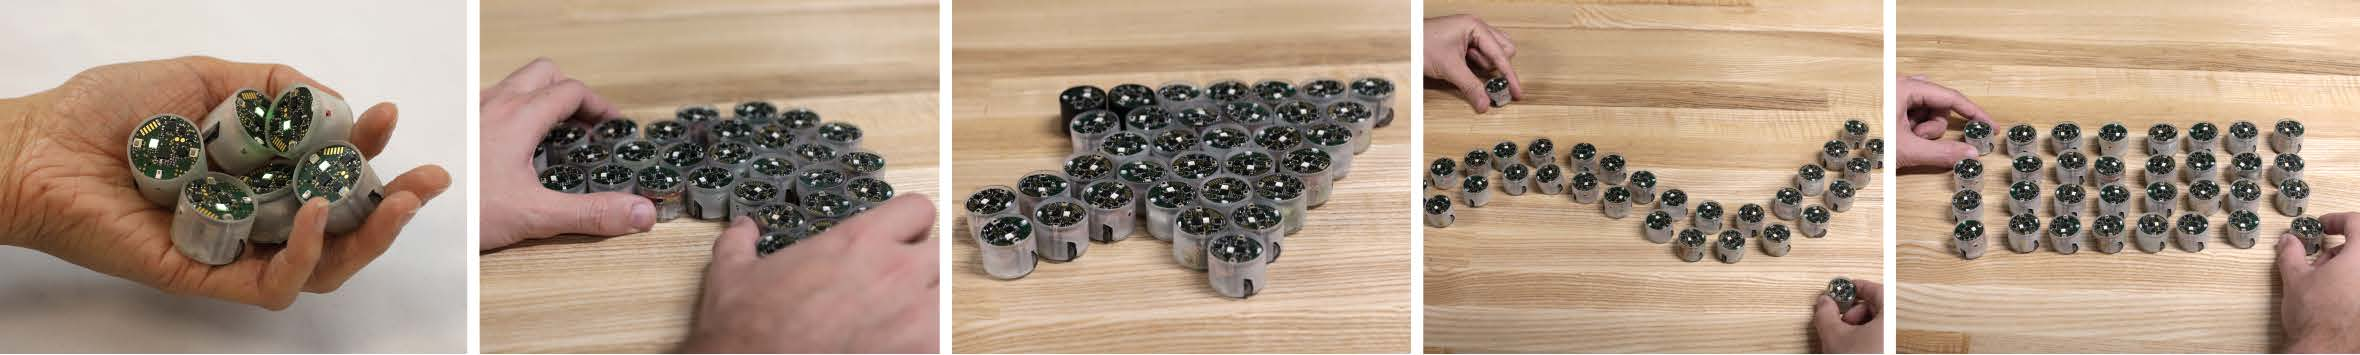
\includegraphics[height=2cm]{zooids-1.jpg}
    \caption*{图~1\hskip1em Zooids可以被持有,可以集体或单独被操纵,表现为物理像素,充当控制器,并且可以在控制下动态移动。 它们是被称为群体交互界面的新型用户界面的积木单元。}
    \label{fig:headfigure}
\end{figure}

{\heiti 摘要:} 本文介绍了集群交互,这是一类新型的人机界面,由许多能够显示和交互的自主机器人组成。我们设计的Zooids是用于开发桌面集群交互的开源软硬件平台。该平台包括一组直径为2.6 cm的定制设计轮式微型机器人,一个无线电基站,一个用于光学跟踪的高速DLP结构光投影仪以及一个用于应用程序开发和控制的软件框架。我们通过使用Zooids开发的一组应用场景说明了桌面集群交互用户界面的潜力,并讨论了集群交互用户界面特有的设计注意事项。

{\heiti 关键词:} 集群用户界面; 实物用户界面。

\section{简介}

本文有助于使伊凡·萨瑟兰(Ivan Sutherland)“一个计算机可以控制物质存在的房间”的终极显示愿景成为现实,以及石井浩史(Hiroshi Ishii)的“人们可以与之交互的能够动态改变形式的新型原子”的愿景[26]。

近来,萨瑟兰(Sutherland)和石井(Ishii)的愿景已迈出了重要的一步,尤其是通过对驱动有形物体[48、50、78]和形状显示[55、56、15]的研究。但是,当前的系统受到许多限制。首先,被致动的桌面有形物品通常仅支持操纵和致动一些(例如3-4)固体物体,这不足以模拟可以改变形状的物理物质。另一方面,形状显示试图获得可以变形和驱动的表面,但是当前的实现并不支持任意的物理拓扑。此外,传统上,两种类型的系统都主要将物理对象用作输入,而输出几乎总是通过单独的基于像素的显示技术来提供。尽管视频投影覆盖图允许输入和输出在空间上重合[12],但它们仅提供有限的物理感[5]。同样,许多这样的系统需要笨重的硬件或显示器才能运行,因此主要是要在虚拟环境中运行,而不是嵌入我们自己的物理世界中[24,77]。

我们的研究工作是通过引入Zooid和大量用户界面来填补当前用户界面技术的空白(见图1)。 Zooid是一种硬件和软件系统:具有位置和触摸感应功能的小型轮式机器人,可以通过用户操作和计算机控制自由地布置和重新放置在任何水平面上。

Wikipedia中将“Zooid”定义为“属于动物群体的单个动物。Zooids是多细胞的。Zooids基于群机器人[10,68]的工作,增加了交互性和速度,它们的结构类似于其他孤独动物的结构。群体用户界面是使用自我推进的物理对象(例如微型机器人)的集合构建的界面,这些对象可以共同移动并对用户输入做出反应。群体用户界面可以看作是Sutherland和Ishii基于可编程物质的用户界面的未来派愿景的粗粒度版本。

由于Zooids具有在空间上自由,快速地重新配置自身的能力,因此,Zooids的集合可以充当显示器并提供有意义的用户输出。由于它们能够感知用户的动作,因此动物小动物还可以支持丰富的输入。例如,用户可以使用“扫动”手势一次移动Zooids,或者一次操纵许多Zooids[35]。可以在应用程序端实现复杂的交互行为,例如,动物类可以充当控件或操纵其他动物类的句柄;他们甚至可以移动其他轻型物体。同时,由于所有输入和输出都可以通过相同的物理元素进行调节,因此该系统能够实现输入和输出之间的完全融合,并提供物理操作的完整体验。最后,该系统相对轻巧,仅需使用紧凑的DLP投影仪(122毫米115毫米48毫米)进行光学跟踪。动物类动物可以在任何水平表面上操作(例如,一张纸,凌乱的办公桌,餐桌或游戏板),从而可以将大量的用户界面与日常的物理环境融合在一起。为了刺激对群体用户界面的未来研究,我们以开源和开放硬件的形式分发了Zooids桌面群体用户界面平台。

总而言之,我们的贡献是:

\begin{itemize}
    \item 群体用户界面的有效定义,包含多个已实现的示例,
    \item 第一个用于实验桌面群用户界面的开源硬件/软件平台,
    \item 一组场景来说明我们的系统和桌面群体用户界面通常提供的前所未有的可能性,
    \item 关于群体用户界面的一些一般设计原理和设计挑战的讨论。
\end{itemize}

此外,Zooids有以下优点:

\begin{itemize}
    \item 与先前启动的有形用户界面可以共存,
    \item 既可以充当单个对象,又足够小以充当物理显示器的“像素”,
    \item 可以单独或集体操作,包括使用标尺等物理工具,
    \item 重量轻,可以在任何水平表面上操作,并且具有较低的成本:现在每个约50美元,如果批量生产,则为20美元。
\end{itemize}

\section{背景}

我们的工作涉及几个研究领域,即:桌面有形用户界面,形状显示,群机器人和数据物理化。

\subsection{桌面有形用户界面}

尽管有形用户界面(TUI)有许多不同的形式(包括传感器和执行器的模块化组件[19,40]),但桌面TUI尤其常见。

桌面TUI允许用户通过移动平面桌面上的物理对象(有形)与数字信息进行交互[72,73]。这些系统已用于一系列应用,例如系统工程控制[51],音乐作品[52],城市规划[74]和教育[23]。

传统桌面TUI的一个局限性是数字对象与物理对象之间的单向映射-如果前者发生变化,后者可能会变得不一致[26]。已经提出了许多技术来激活有形物体,包括2D门架[6,38],电磁体阵列[48,50,78、76],超声波换能器阵列[42],静电的吸引力[80,4],振动[57,81]和移动机器人[60,30、58、47、43、53、49]。这些系统还通过多种方式支持位置跟踪,例如使用LED或标记的摄像头(包括使用光学多点触摸台的摄像机)进行光学跟踪或基于投影仪的跟踪。有形物品的大小从硬币大小[48]到10厘米[53]不等。

人们已经在可动的桌面TUI上探索了多种交互技术,主要是基于每只手的单个有形物体的直接操纵[48],或者通过多点触摸输入[53]对小群可移动物体的直接操纵。 Patten [50]探索了将被动工具与可驱动有形物体结合使用来指定计算约束。其他研究人员在驱动的有形物体上增加了垂直位移等尺寸[43]。这些有效的有形物体在互动时可以通过在用户的手沿表面平移时直接对其施加力来提供触觉反馈[48、41]。由于远程对象可以保持同步[6,58],因此驱动的TUI还为远程协作提供了机会。

桌面TUI的设计空间很大,已经进行了很多探索。但是,先前的系统尚未考虑与许多(例如10、30或更多)小的驱动有形物体进行交互,我们展示了这种交互作用为新颖的交互作用和应用打开了可能性。同样,在许多以前的系统中[48、50、60、58、47、43、53、49、81],有形与图形显示结合使用,因此,有形主要用作数字信息的句柄。我们对用户界面感兴趣,在用户界面中,有形实体不仅用作控制器,还用作数字内容的表示。

\subsection{实体显示和可编程物质}

形状显示是涉及物理表面或体积的用户界面,可以感知用户输入,并且其几何形状可以由计算机控制[56,61]。许多此类系统支持使用电动棒[54、39、15]阵列对2.5D表面进行离散形状控制,而其他系统则支持使用气动或液压致动[14、82]或形状记忆合金进行连续形状控制[61]。当前,这些系统中的许多系统需要重型设备,并且仅允许对物理几何形状和拓扑进行有限的控制。特别是,以前的系统都无法模拟单独的,分离的物理对象。

这些研究工作部分地受到了Sutherland和Ishii之前讨论的愿景的启发,在这些愿景中,计算机将能够重新配置物理物质以重建任何物理形状。机器人技术和材料科学等其他领域也对实现“可编程物质”的梦想感兴趣,但到目前为止,大多数进展仅是理论上的[18,64]。工作原型依赖于群体机器人技术,我们将在后面讨论。

\subsection{集群机器人}

群体机器人是从自然群体中提取的,在自然群体中,鸟类或蚂蚁等社交动物可以根据简单的规则通过相互移动和交互来产生复杂的集体行为。迄今为止,已实施的最大的机器人群包括多达1,000台机器人,尽管它们移动缓慢(约1厘米/秒,而动物群的速度约为50厘米/秒)[63]。我们的论文是从过去对群体机器人技术的研究中得到启发的[10,9],但是尽管群体机器人技术领域一直最关注如何使用分布式智能和完全自治的代理来模仿群体行为,但我们专注于与机器人的直接物理交互。小群机器人,HCI应用程序,并采用集中式系统来协调机器人。

机器人技术的研究人员已开始开发与群体机器人进行交互的方法,但大多数方法仅在鼠标操作的计算机模拟中进行了测试[29,31]。阿隆索-莫拉(Alonso-Mora)及其同事研究了群体机器人作为物理显示器的用途[2],最近扩展了他们的系统,以通过素描[21],手持平板输入[20]和空中手势[3]支持交互。他们的系统与Zooids共享许多功能,但我们的论文重点是对群体机器人进行直接的有形操纵,并探讨了更广泛的应用场景。

最近,Rubens等人[62]描述了一种基于无人机的空中3D物理显示系统,用户可以通过直接操纵无人机进行交互。尽管他们的目标是最终收敛到群体用户界面,但是每架无人机都很大(8.9厘米),并且由于湍流问题,可同时使用的无人机数量受到限制-他们的原型机目前由3架无人机组成。无人驾驶飞机100 [16]项目涉及一百个称为“垃圾桶”的无人机。每个都有灯光,可以在三个维度上定位,从而形成了能够显示动态图像的编排群。但是,较大的操作量会阻止直接操作。

\subsection{数据实体化}

基于围绕体现和分布式认知的认知科学研究,最近对围绕物理数据可视化的信息可视化领域产生了兴趣[28,25,84]。 研究人员已经表明,被动的数据物理表示形式可以促进参与度[45],更好地支持数据解释[27]和视力障碍[36]。

较少的工作探讨了动态物理可视化,因为它们的构建更加复杂[28],但是最近的工作已经研究了使用2.5D形状显示进行数据解释[71]。 但是,可用于2.5D形状显示的可视化技术范围有限。 Swarm界面为将许多传统的2D信息可视化以及更新的交互式数据可视化物理化提供了一个有前途的平台[83,44]。

\subsection{集群用户界面}

我们建议将群体用户界面(swarm UI)称为:

“人机界面由独立的自走元件组成,它们共同移动并对用户输入做出反应”。

独立的:用户界面元素需要相互物理分离并可以自由移动。反例包括计算机显示器上的图形元素,它们都是单个物理对象的一部分。铰接式模块,2.5D形状显示器[15]和物理控制面板(如调音台)也不合格,因为活动部件和控件已连接且不能随意移动。

自走式:元素需要能够在没有外力的情况下移动。反例包括被动物理令牌[25,34]。

集体运动:从定义上讲,群体行为涉及集体运动。因此,这些元素需要能够通过相互交换信息或与中央协调器进行信息协调移动。另外,用户界面包含的元素越多,他们的动作就越有资格被归为集体,因此界面越“像群”。

对用户输入做出反应:这些元素需要感知用户输入并对此输入做出反应。因此,大多数群体机器人系统不是群体用户界面,因为它们缺少用户交互元素。根据我们的定义,交互式显示的显示屏只能接收来自外部资源(例如鼠标或键盘)的用户输入,根据我们的定义,它也不是显示屏用户界面,因为元素本身需要能够对用户输入做出反应。使用计算机视觉检测空中手势的系统(例如DisplaySwarm [3])位于灰色区域。为了实现流畅的交互,系统的速度至关重要:群集用户界面的元素必须足够快才能以可用的速率发生形状变化。理想的过渡时间大约为一秒,因为这大约是系统被认为是交互式的极限[46],也是在常规图形显示上进行动画过渡的推荐持续时间[22]。

根据我们的定义,最接近群体用户界面的系统是自走有形物品[60、30、58、47、43、53、49]和BitDrones [62],因为它们是由独立的自走物品制成可以以协调的方式移动并可以直接操纵的元素。但是,这些系统只涉及很少的元素(即大约4-5),因此最好是实际群体用户界面的低保真原型。尽管许多此类系统可能涉及更多的单元,但外形小巧(例如,动物类动物比Rosenfeld的[60]机器人小3倍以上)可以实现各种类型的交互。用户可以一次操纵许多类动物,而几十个大型机器人甚至可能不适合放在普通桌子上。此外,以前的工作没有讨论或演示大量的用户界面,这是我们的重点。

原则上,群体用户界面可以采用多种形式,并且可以以多种不同方式实现。例如,大量的UI可以由自由浮动的粒子[66]或
 
可以在3D空间中自由移动的无人机[62],或者可以由在2D表面上演化的物体组成[48]。在本文中,我们专注于在2D曲面上移动的元素,即桌面群体用户界面。接下来,我们讨论动物模型的实现,然后通过使用动物模型实现的示例说明桌面群体接口提供的可能性。

\section{使用Zooids的SWARM UI示例}

在本节中,我们将在解释其软硬件设计之前,通过简单的用例和场景来说明和讨论Zooids提供的可能性。 大多数示例也可以在随附的视频中看到。

\subsection{集群绘图}

\begin{figure}[htbp]
    \centering
    \includegraphics[height=8cm]{zooids-2.png}
    \caption*{图~2\hskip1em 徒手画图(1-3)和曲线操作(4)}
\end{figure}